\section{The global climate impact of aviation}
\label{climate}
Aircraft emissions induce climate effects by perturbing the flux of inbound shortwave (SW) solar radiation and outbound longwave (LW) terrestrial radiation emitted from the Earth's surface through absorption and scattering processes that give rise to warming or cooling of the atmosphere \cite{Myhre2013}. Climate metrics such as radiative forcing can be used to measure the climate contribution of each individual emission species, enabling the determination of the net global warming effect from aviation. This section explores the potential global impact of aviation deduced from measurement and modelling of atmospheric processes.

%Accurate quantification of aviation's climate impact requires sufficient modelling of plume-scale effects that are neglected in global models. The accumulation of aircraft emissions in high-density flight regions can lead to saturation effects which affect aviation's net warming effect. This section elaborates on the literature associated with these research areas, to help the reader conceptualise why the atmospheric response to aircraft emissions is dependent on background ambient conditions, and hence why it is also influenced by the presence of other aircraft exhaust plumes in close vicinity.

\subsection{Aircraft emissions in the Upper Troposphere and Lower Stratosphere}
As figure \ref{FB_dist_spatial} suggests, the vast majority (\textasciitilde60\%) of aviation fuel burn and hence aviation emissions, occur at cruise altitudes, between 9 and 13~km vertically. The region of the atmosphere encompassing this volume of airspace is known as the Upper Troposphere and Lower Stratosphere (UTLS), with bounds of $\pm$5~km above and below the conventional tropopause \cite{Gettelman2011}. Around 20--40\% of total aircraft emissions are released in the LS \cite{IPCC1999, Hoinka1993} and the rest are released in the troposphere, extending from the surface at take-off to the UT at aircraft cruise altitudes. The greenhouse effect due to the release of chemically-active substances in the UTLS is considerably greater than that of emissions at the surface. This is because the climate in the UTLS is more sensitive due to increased residence times of pollutants, lower background concentrations (meaning emissions have a greater influence on the atmospheric chemistry), lower temperatures which drive reversible reactions in an unfavourable direction, and finally, a higher radiative efficiency which gives rise to more efficient photochemistry \cite{Schumann1997}. Johnson et al.\ (1992) \cite{Johnson1992} further validates this claim, with model results concluding that \ce{NO_x} emissions constitute a 30 times greater climate impact in the UT compared to equivalent surface emissions, due to the absence of direct deposition and slower conversion to stable reservoir species at aircraft cruising altitudes.

Despite such a large proportion of air traffic emissions being released into the LS region, it is thought that the perturbation to the chemical and radiative state of the stratosphere is negligible, as the vast majority of species emitted into the stratosphere are transported downwards into tropospheric regions, where they interact with the atmosphere there \cite{Lee2010, Grewe2002, Forster2003}. Henceforth, this review will primarily focus on the tropospheric response to aircraft emissions, except for water vapour, where the stratospheric climate response becomes particularly noteworthy.

\subsection{Radiative forcing of aircraft emissions}
High altitude emissions from aviation impact the climate through a variety of climate forcing pathways. Some greenhouse gases such as \ce{CO_2} and \ce{H_2O} are emitted directly, others are produced indirectly through chemical processing of aircraft emissions, such as the reaction of \ce{NO_x} with atmospheric trace species to catalyse ozone production and methane destruction. Water vapour and PM emissions are responsible for the formation of high ice clouds known as condensation trails (contrails), which often trap outbound LW radiation within the atmosphere more efficiently than they reflect inbound SW radiation. PM emissions also have the potential to induce a climate perturbation through direct radiative processes due to aerosols, which may warm or cool the climate depending on the particle's optical and microphysical properties \cite{Lee2010}. Diversity in the climate forcing pathways for each emission species means that the only reliable method of determining the severity of each climate contribution is to model the atmospheric response and determine the resulting impact on the radiative flux of the atmosphere \cite{Brasseur1998}.

The most common climate metric used to compare the magnitudes of climate impact from a range of emission species is radiative forcing (RF). RF is defined as the perturbation to the net energy balance of the Earth-atmosphere system due to natural or anthropogenic factors of climate change, measured in watts per square metre [\ce{Wm^{-2}}] \cite{Fuglestvedt2003}. A positive RF means that the climate forcing mechanism is inducing a warming effect and vice versa. Lee et al.\ (2021) \cite{Lee2021} presents an updated analysis of the global effective radiative forcing (ERF) contributions for aviation-induced climate change. ERF is a newly proposed climate modelling framework that builds upon the RF concept by removing rapid atmospheric adjustments that bear no relation to the long-term surface temperature response that occurs over decadal timescales \cite{Myhre2013}. ERF serves as a more suitable equivalency metric to compare the global warming response of heterogeneously distributed short-lived climate forcers and uniformly distributed long-lived climate forcers. Figure \ref{Lee2021} displays the ERF and RF contributions for each of the key aviation-induced climate forcers.

\begin{figure}[H]
  \centering
  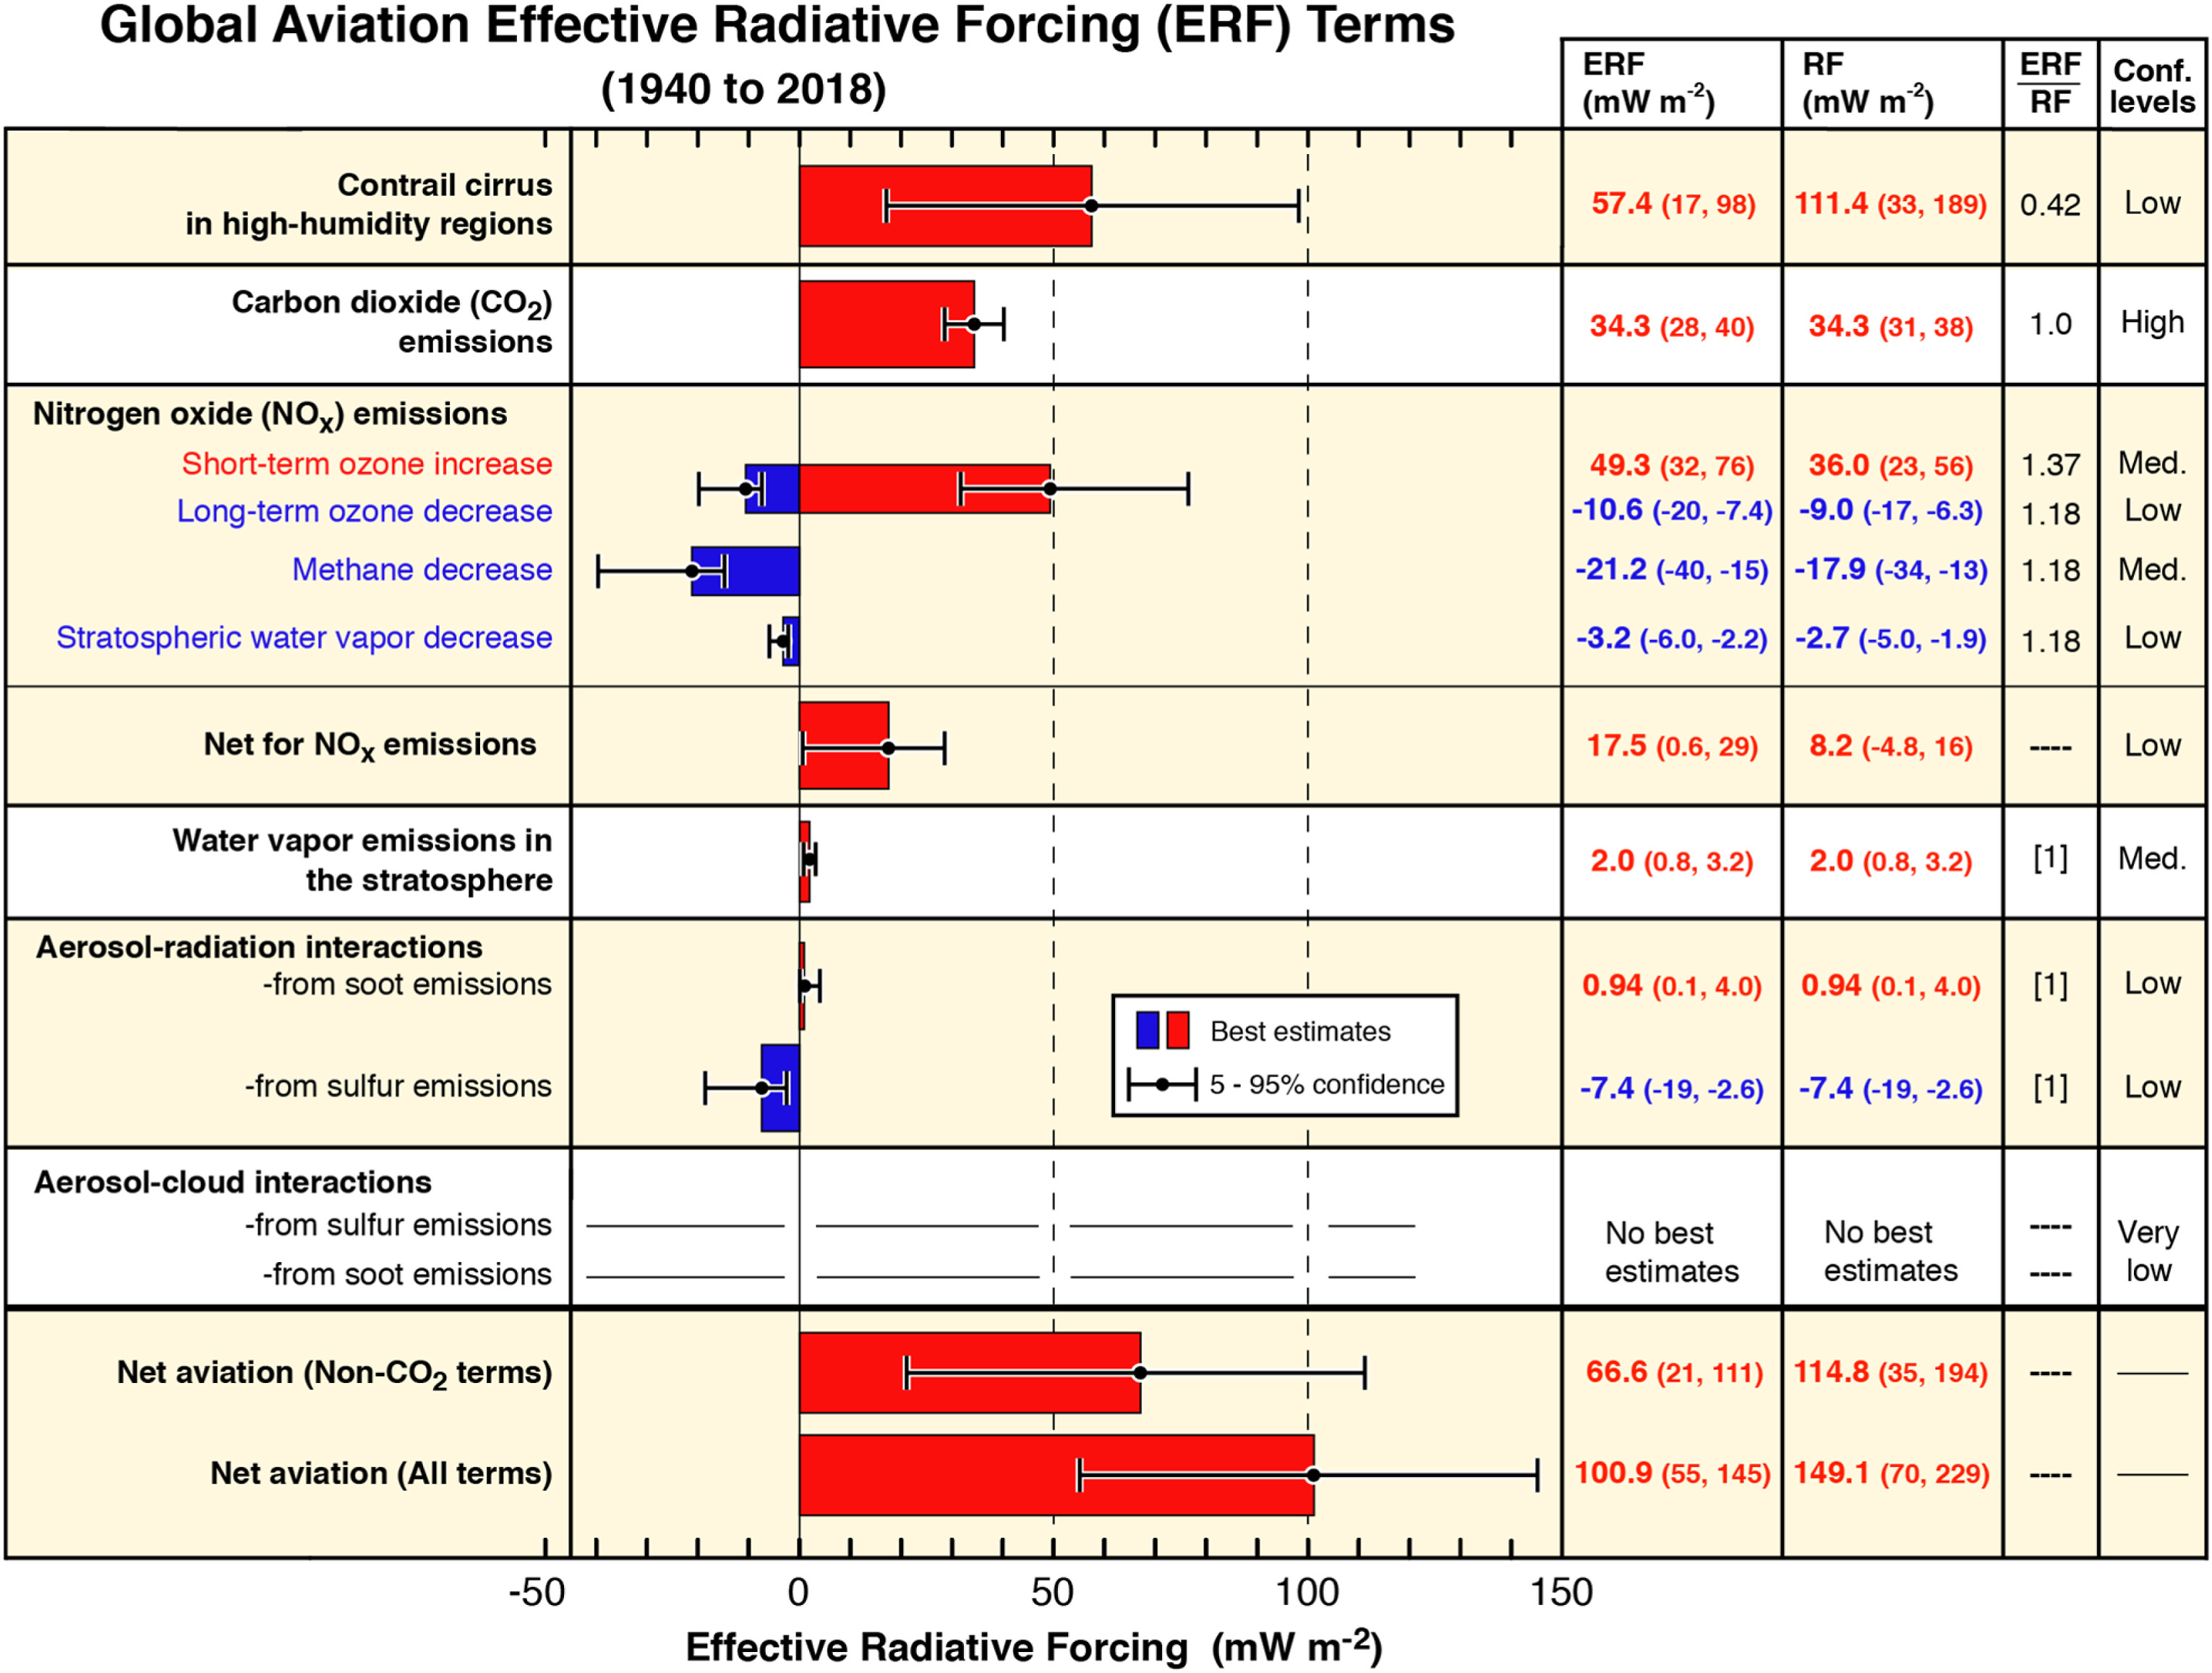
\includegraphics[width=0.9\linewidth]{Lee2021.jpg}
  \caption{Radiative forcing contributions from global aviation between 2000 and 2018 \cite{Lee2021}. Error bars represent 5--95\% confidence interval, with corresponding RF and ERF values shown in parentheses.}
  \label{Lee2021}
\end{figure}

\subsubsection{\ce{CO_2}}
The climatic effects of aviation \ce{CO_2} emissions are direct and well understood, with the thermal absorption of outbound LW radiation leading to warming through the planetary greenhouse effect \cite{Schneider1989}. Carbon dioxide from aircraft constitutes the second largest ERF term in figure \ref{Lee2021} at 34.3~\ce{mWm^{-2}}, and the thermodynamic and photochemical stability of \ce{CO_2} means it has a relatively long atmospheric lifetime, on the order of 100 to 1,000 years \cite{Archer2008}. This means that carbon emissions from aircraft simply serve to increase its atmospheric concentration, leading to the eventual distribution over global spatial scales. The ubiquitous and intuitive nature of \ce{CO_2}-related warming deems it a suitable benchmark to compare warming from non-\ce{CO_2} climate forcers against. The assumption of instantaneous dilution in global models is sufficient for modelling the climate impact due to carbon dioxide, as it exists over vast spatial and temporal scales, meaning the climatic effects occurring on plume time scales are negligible compared with the impact induced over its entire lifetime \cite{Paoli2011}.

\subsubsection{Contrail cirrus}
When emissions of water vapour and PM are released into the aircraft exhaust plume in the cold and moist condition of the UTLS, the water vapour condenses around the particulates due to the high relative humidity (RH), then freezes due to the low external temperatures, permitting the formation of ice crystals. The accumulation of ice crystals in the aircraft wake gives rise to the generation of a condensation trail, also known as a contrail. The evolution of contrails, i.e. how they grow, disperse and persist with time, is largely determined by the ambient conditions of the surrounding atmosphere, with lower temperatures and higher humidities generally leading to more persistent and damaging contrails \cite{Schumann2005}. The formation and persistence of contrails can be predicted purely from the thermodynamic assumption that, as the hot and moist exhaust mixes with the colder and drier ambient air, a contrail will form if the plume exceeds water-saturation at any point and the temperature is low enough for ice nucleation to occur. A contrail will persist in the atmosphere if it mixes with air that is supersaturated with respect to ice, i.e. an ice-supersaturated region (ISSR), growing with time due to deposition of surrounding water vapour onto existing ice crystals \cite{Karcher2018, Schumann2005}. Persistent contrails can sometimes transition to contrail cirrus, either building onto existing cirrus clouds or forming new ones, spreading over vast swathes of the atmosphere \cite{Minnis1998} and inducing significant radiative effects. ISSRs occur frequently at aircraft cruising altitudes and often span hundreds of kilometres horizontally, however only reach depths of 100 to 1,000~m \cite{Spichtinger2016, Dickson2010}. Their shallow nature means that aircraft can avoid them by changing flight level by $\pm$2000~ft to minimise persistent contrail generation for a minor additional fuel penalty \cite{Schumann2011}.

The optical characteristics of contrail ice crystals often exhibit significant levels of opacity, tending to absorb outbound terrestrial radiation more efficiently than they reflect inbound solar radiation. This induces a globally averaged ERF of 57.4~\ce{mWm^{-2}}, meaning, despite their relatively short lifetime in comparison, the current contrail effect contributes more to climate change than the accumulation of aviation carbon, since the dawn of aviation \cite{Burkhardt2011}. Contrail evolution, i.e. how they grow, disperse and persist with time, is largely determined by the ambient conditions of the surrounding atmosphere, with lower temperatures and higher humidities generally leading to a more persistent and damaging contrails \cite{Schumann2005}. The formation and persistence of contrails can be predicted purely from the thermodynamic assumption that, as the hot and moist exhaust mixes with the colder and drier ambient air, a contrail will form if the plume exceeds water-saturation at any point and the temperature is low enough for ice nucleation to occur. A contrail will persist in the atmosphere if it mixes with air that is supersaturated with respect to ice, i.e. an ice-supersaturated region (ISSR) \cite{Karcher2018}. 

%The thermodynamic constraints for contrail formation and persistence were first theorised by Schmidt (1941) \cite{Schmidt1941} and Appleman (1953) \cite{Appleman1953}, based on prior empirical observations \cite{Schumann1997b}, that led to the promulgation of the so-called ``Schmidt-Appleman (SA) criterion". The SA criterion shows that the contrail formation threshold is purely dependent on ambient pressure, relative humidity, and the ratio of water and heat released into the exhaust plume, assuming isobaric mixing between exhaust emission and full dilution into the ambient atmosphere \cite{Schumann1996}. See Tait (2020) \cite{Tait2020} for a detailed description of how the SA criterion can be illustrated on a plot of water vapour partial pressure against temperature. Contrails which surpass water saturation, but do not settle in ice-supersaturated air are generally assumed to be short-lived, as the ice sublimates and deposits into the surrounding atmosphere. However, contrails released into ISSRs, where the ambient humidity is higher than the saturation humidity over ice surfaces, instead grow with time because the ice particles experience deposition of surrounding water vapour molecules \cite{Schumann2005}. Persistent contrails can sometimes transition to contrail cirrus, either building onto existing cirrus clouds or forming new ones, spreading over vast swathes of the atmosphere \cite{Minnis1998} and inducing significant radiative effects. ISSRs occur frequently at aircraft cruising altitudes and often span hundreds of kilometres horizontally, however only reach depths of 100 to 1,000~m \cite{Spichtinger2016, Dickson2010}. Their shallow nature means that aircraft can avoid them by changing flight level by $\pm$2000~ft to minimise persistent contrail generation for a minor additional fuel penalty \cite{Schumann2011}.

%Contrails released into ice-subsaturated air will be short-lived, as the ice particles sublimate in ambient air within a matter of seconds to minutes, meaning the radiative impact is negligible \cite{}. However, contrails released into ISSRs, where the ambient humidity is higher than the saturation humidity over ice surfaces, instead grow with time because the ice particles experience deposition of surrounding water vapour molecules \cite{Schumann2005}. This allows the contrails to persist in the atmosphere for hours and potentially transition into cirrus clouds with vast areal coverage \cite{Minnis1998, }. Persistent contrails and contrail cirrus induce a significant climate impact due to the 

Contrails exhibit radiative forcing through the obstruction of both SW and LW radiative fluxes, with areal coverage and optical depth (opacity) being the key drivers of contrail climate impact \cite{Schumann2017}. A contrail's emissivity (ability to absorb and re-emit infrared LW radiation back towards Earth) and reflectance (ability to reflect inbound SW radiation back out to space due to scattering at visible wavelengths) is a function of contrail optical depth and ice particle microphysics. Contrails and other high ice clouds often warm the climate, as their thin optical depth means partial transparency to solar radiation, whilst their high ice density traps infrared radiation within the atmosphere effectively \cite{Karcher2018}. Contrail RF also displays a distinct diurnal trend; at night, contrails always induce a warming effect, as there is no SW scattering to counteract the LW absorption. During the day, contrails display a reduced net warming effect and perhaps even a net cooling effect, depending on the amount of solar radiation that is redirected back out to space \cite{Newinger2012}. The SA criterion can be used to predict formation and persistence of contrails, however accurate quantification of contrail RF requires sufficiently detailed microphysical modelling, to deduce key information on the underlying formation mechanisms and physical and optical properties the contrail exhibits throughout its evolution \cite{Karcher2015}. See section \ref{Microphysics} for elaboration on the microphysical processes that determine a contrail's radiative characteristics, and how these processes can be parametrised for modelling purposes.

%Contrail EF concept, similar to other climate metrics, takes into account temporal dimension.

\subsubsection{Net-\ce{NO_x}}
Nitrogen oxides (NO and \ce{NO_2}) released from aircraft are not radiatively active and therefore do not induce an immediate climate impact at the point of emission. Their chemical instability does however mean that they exhibit a number of indirect RF effects, due to the chemical reactions that occur following dilution into the ambient atmosphere. The chemical interactions between \ce{NO_x} and trace species in the background atmosphere at aircraft cruising altitudes are highly non-linear and thus, the net-\ce{NO_x} RF contribution is dependent on the instantaneous atmospheric state (time of day and year, latitude, background chemical composition, meteorological situation) \cite{Fritz2020, Kraabol2000b}. 

Emissions of \ce{NO_x} in the troposphere initially leads to the short term local increase in ozone production efficiency (\ce{O_3}) on the time scale of weeks to months. In addition, elevated \ce{NO_x} and \ce{O_3} levels lead to increased hydroxyl radical (OH) production, which in turn, leads to the long term global destruction of ambient methane (\ce{CH_4}) over the time scale of decades \cite{Stevenson2004, Wild2001, Myhre2011}. The short term increase in \ce{O_3} generates a strong positive ERF of 49.3~\ce{mWm^{-2}}, whereas the long term \ce{CH_4} depletion causes a lesser negative ERF of -21.2~\ce{mWm^{-2}} in comparison, however there are a number of secondary negative radiative effects arising from methane depletion that must also be accounted for. This is the reduction in stratospheric water vapour (15\% \ce{CH_4} RF magnitude) and a decrease in long-term background ozone in the troposphere (45\%~\ce{CH_4} RF magnitude), resulting from reduced background \ce{CH_4} concentrations \cite{Holmes2011, Myhre2007}. Despite the long-term negative cooling effects, the short term warming from \ce{O_3} dominates, leading to a largely positive net ERF of 17.5~\ce{mWm^{-2}} overall, as seen from figure \ref{Lee2021}. Section \ref{Gas-phase_photochem} explores the nonlinear \ce{NO_x}-\ce{O_3} relationship further through explanation of the gas-phase photochemical processes that begin in the aircraft plume and are eventually distributed to regional and global scales. 

\subsubsection{Water vapour}
The direct radiative effects induced by aviation water vapour emissions in the troposphere are insignificant, because the influence on background concentrations is negligible when compared with the natural fluxes of the Earth's hydrological cycle \cite{IPCC1999}. Any tropospheric water vapour emissions tend to get lost through deposition, due to high humidity and precipitation in this region, leading to a lifetime of around 9 days. On the contrary, water vapour that is emitted into the stratosphere (without getting transported downwards into the UT) can induce a considerable effect on the surrounding environment, due to extreme dryness at these altitudes \cite{Jensen1996}. This is because increases in stratospheric water vapour (SWV) concentrations impact the climate directly through the greenhouse effect, as well as through influences on the gas-phase and aerosol chemical composition, leading to depletion of ozone and altering the formation and growth of polar stratospheric clouds \cite{Stenke2005}. The combined impact of the direct greenhouse effect and indirect impacts on ozone and polar stratospheric clouds due to increased SWV leads to an overall ERF of 2.0~\ce{mWm^{-2}}.

As proposed in Lee et al.\ (2010) \cite{Lee2010}, the relatively small climate perturbation due to aviation-induced SWV has the potential to increase drastically as future flight concepts begin to take shape. This includes the environmental implications associated with the potential replacement of the current subsonic aircraft fleet with a supersonic high-speed civil transport (HSCT) fleet, that primarily operates in the stratosphere (e.g. \cite{MiakeLye1993, Danilin1994, Grooss1998, Kawa1999}). Furthermore, the prospect of transitioning the entire subsonic kerosene-based commercial fleet to a hypothetical fleet of cryoplanes (hydrogen-powered aircraft with zero carbon emissions) would increase aviation \ce{H_2O} emissions by a factor of \textasciitilde2.5 \cite{Gauss2003}. In the high-humidity conditions of the UT, this brings about the potential for large increases in contrail production, whereas in the LS, this would induce significant perturbations to SWV concentrations.

%However, the present air traffic increases background humidity by less than 1.5\% for regions most frequently used by aircraft. Increased water vapour in the stratosphere also affects the rate of chemical ozone loss, e.g., by increasing the incidence of polar stratospheric clouds.

\subsubsection{Aerosol effects}
Aviation aerosol particles, either emitted directly post combustion, or formed in the wake of the aircraft, can perturb the energy balance of the atmosphere directly, as well as indirectly through the formation of contrail ice particles and heterogeneous chemical processing. The direct aerosol effect is primarily produced by the key non-volatile and volatile PM emissions: soot and sulphate aerosols.

Soot exhibits a direct radiative forcing as it has the strongest absorption of light at visible wavelengths per unit mass, more than any other abundant substance in the atmosphere, thus contributing to global heating through absorption of inbound solar radiation and light rebounded off reflective surfaces such as snow and ice \cite{Bond2013}. The resultant heating of the atmosphere and reduction of sunlight can affect the hydrological cycle and large-scale circulation patterns, having potentially larger implications on the climate than previously thought. Despite its ability to strongly absorb sunlight, aircraft soot is responsible for only a few percent of total atmospheric black carbon, meaning the aerosol-radiation interaction brought about by aviation soot only constitutes a minor ERF of 0.94~\ce{mWm^{-2}}.

Sulphur dioxide (\ce{SO_2}) is formed when sulphur, which is present in hydrocarbon jet fuels, oxidizes during the combustion process \cite{Brown1996}. \ce{SO_2} that is emitted from the aircraft exhaust can be oxidised to form gaseous sulphuric acid (\ce{H_2SO_4}), which may condense on existing particles or contribute to new particle formation in low-condensation environments, resulting in sulphate aerosol formation. Sulphate aerosol is mainly composed of sulphuric acid and corresponding salts such as ammonium sulphate. The optical properties of sulphate mean that it tends to scatter inbound sunlight, thus leading to a net negative (cooling) of 7.4~\ce{mWm^{-2}}, that sways the net direct climate impact of aviation aerosols towards cooling. 

It is relatively well established that aviation-induced aerosols have a direct impact through radiative interactions, as discussed in this section, as well as indirectly through activation of water vapour on PM emissions through contrail formation. There are however, potentially large indirect consequences of aerosol particles interacting with cloud droplets and ambient ice particles nucleation on the aerosol surface. These effects are left without ERF estimates in figure \ref{Lee2021}, as there is great uncertainty around the accuracy of cloud process modelling and the ability to distinguish aircraft-induced clouds and natural clouds \cite{Penner2018}.

\subsection{Global climate modelling}
\label{Climate_modelling}
Quantifying aviation's global climate impact requires the use of computational climate models to predict the atmospheric response to the emission species released by aircraft. Climate models simulate the climate system through mathematical representation of established physical laws (e.g. conservation of mass, energy and momentum) and a plentiful supply of empirical data obtained through real world observation and measurement of physical and chemical quantities (e.g. chemical concentrations, meteorological parameters) \cite{Randall2007}. Gridded aircraft emissions inventories are used as input to climate models \cite{Olsen2013, Wilkerson2010}, in which emissions are homogeneously distributed throughout the entire grid cell that they are released into (i.e. the ID approach). The chemistry, physics and dynamics of the atmosphere are captured in the model, along with the perturbation to the atmospheric state due to emissions, providing an output of the spatial and temporal distributions of chemical species. Radiative transfer schemes can then be used to quantify the climate response to the perturbed chemical composition through instantaneous metrics such as RF and ERF. The variability in chemical and radiative properties of climate forcing species does however vary considerably with time. For example, \ce{CO_2} is distributed globally and affects the climate gradually over centuries, whereas contrails induce a severe yet short-lived, localised radiative impact \cite{Lee2021}. Therefore, metrics such as Global Warming Potential (GWP, GWP*) and Global Temperature Potential (GTP) have been developed to better account for the temporal variation of certain properties, providing a more well-rounded analysis of the climate contributions of aircraft emission species \cite{Fuglestvedt2003, Fuglestvedt2010, Cain2019}.

There are two main climate model distinctions for use in aviation climate modelling: general circulation models (GCMs) and chemistry-transport models (CTMs). GCMs are highly sophisticated, yet very complex, as they are what are known as ``online'' models, calculating chemical composition, temperature and transport circulation simultaneously and in real time. This is often computationally expensive and may require very long processing times to run, depending on the simulation. CTMs on the other hand are reduced order ``offline'' models, calculating chemical composition based on pre-determined GCM results or empirically observed temperature and transport circulation data \cite{IPCC1999}. Example usage of GCMs in aviation climate modelling include the European Centre HAmburg Model (ECHAM) \cite{Stevens2013} for analysis of future contrail cirrus radiative forcing \cite{Bock2019} and the Community Atmosphere Model version 5 (CAM5) \cite{Neale2004} to comprehensively represent aviation aerosol climate impact \cite{Gettelman2013}. CTMs appear much more frequently in the literature due to their versatility and computational efficiency. For example the UK Meteorological Office CTM STOCHEM \cite{Cooke2010} coupled with the Common Representative Intermediates (CRI) chemical mechanism \cite{Jenkin2008} is used for modelling the global impact of aviation \ce{NO_x} emissions on ozone production \cite{Wasiuk2014}, MOZART CTM \cite{Emmons2010} for use in investigating the trade-off between \ce{CO_2} and \ce{NO_x} emissions \cite{Freeman2017}, and another six CTMs are presented in \cite{IPCC1999} for aviation climate impact modelling purposes. Various model intercomparison studies provide an up-to-date, elaborate review of the models available for UT and LS (and thus aviation) climate modelling \cite{Roelofs2003}. 


%Climate models provide a realistic quantitative estimate of future climate change especially at the continental scale. In recent years, various climate models have been developed to improve understanding of climate processes and to perform more realistic time-dependent simulations of climate change. These models can incorporate physical processes in greater complexity such as coupling of climate system components and enhanced model resolution. The most sophisticated climate models are the General Circulation Models (GCMs) coupled with the chemistry scheme which can be used to study the potential anthropogenic influences on current and future climate \cite{Solomon2007}. However, the GCMs are very complex and computationally expensive, therefore may need very long processing time to run (depending on the climate perturbation) on a high-performance computer. To overcome this, simple climate models (SCMs) are used for estimating future climate impacts of aviation activity which are generally parameterized to reproduce the main characteristic responses of GCMs.

%SCMs are known as reduced complexity model, computationally inexpensive and widely used decision support tools for the policy makers. SCMs are used to evaluate climate impacts from a wide range of sources, from total anthropogenic emissions to sectoral emissions (e.g., aviation emissions). Model for the Assessment of Greenhouse Gas Induced Climate Change (MAGICC) is one of the SCMs which is not specific to aviation and can be used in different emissions scenarios to estimate time-dependent concentrations, radiative forcing, temperature response and sea-level rise from different perturbations \cite{Meinshausen2011}. Linear climate response model (LinClim) is a very effective SCM which has been customised specifically for aviation purposes. It implements a single impulse response function that is calibrated against more sophisticated parent GCM model. The global aircraft fuel emissions derived from emissions database and the calculated emissions indices are used to calculate historical, present day and future emissions trends of CO2, NOx, water vapour, sulphate and black carbon aerosols. LinClim calculates the climate impacts from non-CO2 species and contrails by scaling the emissions or distance travelled to an externally calculated base year radiative forcing. The carbon cycle in LinClim is based on the Maier-Reimer and Hasselmann (1987) \cite{} model and the CO2 RF is calculated using the function applied in IPCC AR468 \cite{Solomon2007}. The temperature response can be calculated by LinClim using radiative forcing and climate model parameters that are parameterized to LinClim’s parent GCM.

%The impact of the species released from aircraft on the atmosphere is non-linear. Thus, a non-linear climate-chemistry response model, AirClim \ce{Grewe2008} applicable to aviation industries is developed. This model comprises a linearisation of atmospheric processes from the emissions and productions of \ce{CO_2}, \ce{H_2O}, \ce{CH_4}, \ce{O_3} and contrails to radiative forcing, resulting in an estimate of surface temperature change.

%The FAA Aviation Environmental Portfolio Management Tool (APMT) uses impulse response models along with a simplified energy balance model to give aviation impacts for CO2, NOx on methane, NOx on ozone, sulphates, soot and contrails/contrails cirrus in terms of radiative forcing and global temperature change \cite{Marais2008}.





%\subsubsection{Instantaneous dispersion (ID)}
%Convention amongst the climate modelling community is to assume instantaneous dispersion (ID) of aircraft emissions into the dimensions of the latitude-longitude-altitude grid cell, whose size is determined by the model resolution. This ID assumption therefore neglects the presence of aircraft plume, and hence does not capture the aforementioned aircraft-induced dynamics which have a notable influence on the ensuing chemical and physical response of the atmosphere in real life \cite{}. Due to the lack of plume representation, ID modelling can be effected through simple analysis of the production and loss rates of an emission species, subject to instantaneous input of emissions concentrations at the time of release.


%Tropospheric chemistry is dominated by ozone (\ce{O_3}), a potent greenhouse gas which contributes to climate change and air quality issues. \ce{O_3} is an oxidant in its own right, reacting with reactive volatile organic compounds (VOCs, see later) but is the precursor to the OH radical, which is known as the chemical detergent of the lower atmosphere. The OH radical reacts with VOCs and allows them to be oxidised and removed from the atmosphere. Photolysis of ozone (absorption of sunlight in the UV region ~ 290-330 nm and the breaking of an O-O bond) starts the process of OH production, depicted by reaction (1), where hv denotes a photon of light;

%\begin{equation}
%	\ce{O_3 + hv -> O(^{1}D) + O_2}
%	\label{O3toO1D}
%\end{equation}
%
%Reaction \eqref{O3toO1D} makes a reactive oxygen atom \ce{O(^{1}D)}, that can either collide with N2 or O2 molecules (denoted as M) and be quenched to ground state \ce{O(^{3}P)} atoms in reaction \eqref{O1DtoO3P}
%
%\begin{equation}
%	\ce{O(^{1}D) + M -> O(^{3}P) + M}
%\label{O1DtoO3P}
%\end{equation}
%
%Or it can react with water to form HO radicals
%
%\begin{equation}
%	\ce{O(^{1}D) + H_2O -> OH + OH}
%\end{equation}
%
%OH radicals can then participate in chemical cycles that preserve levels but also remove pollutants, CO, in the following examples. First, under clean conditions (low \ce{NO_x} = NO and \ce{NO_2}) the following scheme (1) takes place:
%
%\begin{equation}
%	\ce{OH + CO -> H + CO_2}
%\end{equation}
%
%\begin{equation}
%	\ce{H + O_2 + M -> HO_2 + M}
%\end{equation}
%
%\begin{equation}
%	\ce{HO_2 + O_3 -> OH + 2O_2}
%\end{equation}
%
%Net reaction \ce{CO + O_3 -> CO_2 + O_2}
%
%Here, ozone is removed and CO is oxidised to form \ce{CO_2}, which, in a pre-industrial world, was taken up by plants and the oceans on relatively short timescales. This clean condition scheme removes pollutants and keeps ozone levels under control. However, industrial activity through fossil fuel combustion has increased levels of \ce{NO_x} in the atmosphere, changing from scheme (1) to scheme (2):
%
%\begin{equation}
%	\ce{OH + CO -> H + CO_2}
%\end{equation}
%
%\begin{equation}
%	\ce{H + O_2 + M -> HO_2 + M}
%\end{equation}
%
%\begin{equation}
%	\ce{HO_2 + NO -> OH + NO_2}
%\end{equation}
%
%\begin{equation}
%	\ce{NO_2 + hv -> NO + O(^{3}P)}
%\end{equation}
%
%\begin{equation}
%	\ce{O(^{3}P) + O_2 + M -> O_3 + M}
%\end{equation}
%
%Net reaction: \ce{CO + 2O_2 -> CO_2 + O_3}
%
%Now, ozone is formed as CO is oxidised, and one can assume that adding more \ce{NO_x} would further increase ozone production. However, if NO and \ce{NO_2} levels surpass a threshold, they can compete with VOC for reaction with OH radicals:
%
%\begin{equation}
%	\ce{OH + NO + M -> HONO + M}
%	\label{HONO}
%\end{equation}
%
%\begin{equation}
%	\ce{OH + NO_2 + M -> HNO_3 + M}
%	\label{HNO3}
%\end{equation}
%
%Reactions \eqref{HONO} and \eqref{HNO3} are called termination reactions, removing radicals from the atmosphere and preventing \ce{O_3} formation. 
%
%% Ozone NOx curve here

